\documentclass[conference]{IEEEtran}
\IEEEoverridecommandlockouts

\usepackage{cite}
\usepackage{amsmath,amssymb}
\usepackage{graphicx}
\usepackage{booktabs}
\usepackage{array}
\usepackage{multirow}
\usepackage{xcolor}
\usepackage{listings}
\usepackage{tikz}
\usetikzlibrary{positioning,arrows.meta,fit,calc}
\usepackage[hidelinks]{hyperref}
\usepackage{url}

\newcommand{\benchSpeedupMin}{225}
\newcommand{\benchSpeedupMax}{878}
\newcommand{\benchOverheadMin}{29}
\newcommand{\benchOverheadMax}{217}
\newcommand{\benchCPU}{Intel Xeon Processor @ 2.10GHz}
\newcommand{\benchCC}{13.3.0}
\newcommand{\benchPython}{3.13.16}
\newcommand{\benchAllMatch}{all outputs matched}

% Primitive \input, so generated table rows can be read inside a tabular
\makeatletter
\newcommand{\inputrows}[1]{\@@input #1 }
\makeatother

% ---------------------------------------------------------------- listings
\definecolor{kw}{HTML}{1F3A93}
\definecolor{ty}{HTML}{6A2C91}
\definecolor{cm}{HTML}{5F6368}
\definecolor{st}{HTML}{1B6B3A}
\lstdefinelanguage{cmm}{
  morekeywords={module,fn,main,let,mut,if,else,while,do,for,print,true,false,return,switch,case,default},
  morekeywords=[2]{int,float,bool,string,array,list,stack,queue},
  sensitive=true,
  morecomment=[l]{//},
  morecomment=[s]{/*}{*/},
  morestring=[b]",
}
\lstset{
  basicstyle=\ttfamily\footnotesize,
  keywordstyle=\color{kw}\bfseries,
  keywordstyle=[2]\color{ty},
  commentstyle=\color{cm}\itshape,
  stringstyle=\color{st},
  columns=fullflexible,
  keepspaces=true,
  frame=lines,
  framesep=3pt,
  xleftmargin=3pt,
  xrightmargin=3pt,
  aboveskip=6pt,
  belowskip=4pt,
  captionpos=b,
  showstringspaces=false,
  literate={--}{{-{}-}}2,
}
\lstdefinestyle{diag}{language={},basicstyle=\ttfamily\fontsize{6.6}{7.6}\selectfont,keywordstyle={},literate={},
  breaklines=true,breakatwhitespace=true,postbreak=\mbox{\hspace{1.2em}}}
\lstdefinestyle{plain}{language={},basicstyle=\ttfamily\fontsize{7}{8.2}\selectfont,keywordstyle={},literate={--}{{-{}-}}2,
  breaklines=true,breakatwhitespace=true}

\newcommand{\cmm}{C\texttt{-{}-}}
\newcolumntype{L}[1]{>{\raggedright\arraybackslash}p{#1}}

\begin{document}

\title{\cmm{} (C Minus Minus): Design and Implementation of a Memory-Safe Imperative Language, Compiler, and
Web-Based Compiler Studio\\[6pt]
\large Project Report\\[2pt]
\normalsize Supervised by Prof.\ Hariharan R L, Center for AI Research, School of Computer Science and Engineering (SCOPE)}

\author{
\IEEEauthorblockN{Ronit Mexson}
\IEEEauthorblockA{\textit{School of Computer Science and}\\
\textit{Engineering (SCOPE)}\\
Reg.\ No.\ 24BAI0036}
\and
\IEEEauthorblockN{Mit Kumar Raju Panchal}
\IEEEauthorblockA{\textit{School of Computer Science and}\\
\textit{Engineering (SCOPE)}\\
Reg.\ No.\ 24BAI0279}
\and
\IEEEauthorblockN{Garv Gupta}
\IEEEauthorblockA{\textit{School of Computer Science and}\\
\textit{Engineering (SCOPE)}\\
Reg.\ No.\ 24BDS0169}
}

\maketitle

\begin{abstract}
This report presents the design, implementation and evaluation of \cmm{} (C Minus Minus), a statically
typed, C-like imperative programming language built on the principle of \emph{safety by removal}. Rather than
adding garbage collection, ownership tracking or runtime sanitizers to make dangerous features safe, \cmm{}
removes the features themselves: there are no pointers, no null, no uninitialized variables, no implicit
conversions and no undefined behaviour. Bindings are immutable by default, collections have deep-copy value
semantics, and every remaining fault is a deterministic, positioned runtime trap. The project delivers a
complete toolchain written in pure Python with no external dependencies: a lexer, a recursive-descent
parser, a semantic analyzer, a reference interpreter, an ISO~C99 transpiler, a diagnostics system with 60
documented error codes, a command-line tool, a VS~Code extension, and a server-rendered web compiler studio
with live diagnostics. The report describes each component, the 445-test quality-assurance process run on
three operating systems, the deployment, and an evaluation of safety and performance, including a case study
that uses \cmm{} to model AVX-512 vector predication.
\end{abstract}

\begin{IEEEkeywords}
programming language design, memory safety, compiler construction, static analysis, interpreters,
source-to-source translation, compiler diagnostics, web-based development environments
\end{IEEEkeywords}

% ======================================================================
\section{Introduction}
% ======================================================================
\IEEEPARstart{C}{} and C++ remain the foundation of operating systems, embedded software and performance-critical
applications, but their raw pointers, manual memory management and long list of undefined behaviours make
them the leading source of severe security defects. Microsoft reports that about 70\% of the vulnerabilities
it assigns a CVE each year are memory-safety issues~\cite{miller2019}, the Chromium project reports a similar
share among its serious security bugs~\cite{chromium_memsafety}, and government agencies now ask software
vendors to publish memory-safety roadmaps~\cite{cisa2023}.

Memory-safe alternatives exist, but each adds complexity: garbage-collected languages add a runtime, and Rust
adds ownership, borrowing and lifetimes that beginners find hard to learn~\cite{rust}. This project asks a
different question: \emph{what is left of C's simple, explicit style if every construct capable of undefined
behaviour is removed instead of guarded?} The answer is \cmm{}, a language small enough to learn quickly and
to implement completely within a student project, yet strict enough that the most common classes of
memory-corruption and arithmetic defects either cannot be written or stop the program with a clear message.

\subsection{Objectives}
\begin{enumerate}
  \item Design a statically typed imperative language whose grammar and type system exclude null, pointers,
        uninitialized reads, implicit narrowing and undefined behaviour.
  \item Specify the language normatively, down to exact error messages, number formats and source positions,
        so that every behaviour is testable.
  \item Implement a complete, dependency-free toolchain: front end, reference interpreter and a C99 back end.
  \item Make diagnostics understandable to beginners, with explanations, fixes and spelling suggestions.
  \item Provide tooling for adoption: a CLI, an editor extension and a browser-based compiler studio.
  \item Validate the implementation with automated tests on Windows, macOS and Linux, and evaluate its
        safety and performance.
\end{enumerate}

\subsection{Scope and organization}
Version 0.2.0 of \cmm{} is covered. Section~\ref{sec:lit} reviews related work and Section~\ref{sec:req}
states the requirements. Section~\ref{sec:arch} gives the system architecture, Section~\ref{sec:lang} the
language, and Section~\ref{sec:impl} the compiler implementation. Sections~\ref{sec:diag}--\ref{sec:web}
describe the diagnostics, the developer tooling and the web studio. Section~\ref{sec:qa} covers testing and
deployment, Section~\ref{sec:eval} the evaluation, and Section~\ref{sec:future} limitations and future work.

% ======================================================================
\section{Literature Survey}\label{sec:lit}
% ======================================================================
\textbf{Safe dialects of C.} Cyclone~\cite{cyclone} keeps C's syntax but restricts pointer arithmetic and adds
region-based memory management with several pointer kinds. CCured~\cite{ccured} infers pointer kinds for
legacy C and inserts run-time checks. Checked~C~\cite{checkedc} adds checked pointer and array types that
can be adopted incrementally. All three keep pointers and must therefore track them; \cmm{} removes them.

\textbf{Ownership-based safety.} Rust~\cite{rust} guarantees memory safety without a garbage collector
through ownership, borrowing and lifetimes. \cmm{} achieves alias freedom far more simply, if less
efficiently, by giving collections value semantics.

\textbf{Dynamic detection.} AddressSanitizer~\cite{asan} instruments C and C++ programs to detect
out-of-bounds and use-after-free accesses during testing, but offers no guarantee in production.

\textbf{Language subsets.} MISRA~C~\cite{misra} restricts C through coding rules checked by external tools,
and SPARK~\cite{spark} restricts Ada so that programs can be formally verified. \cmm{} follows the same
subsetting philosophy but makes the restrictions part of the language itself.

\textbf{Compiler diagnostics.} Studies of novice programmers find terse compiler messages a major
obstacle~\cite{becker2019}; Elm popularized messages written for humans~\cite{elm_errors}. \cmm{} applies this
style to every diagnostic and adds spelling suggestions based on edit
distance~\cite{damerau,levenshtein}.

\textbf{Compiler construction.} The implementation follows classical techniques: hand-written scanning,
recursive-descent parsing by precedence levels, and syntax-directed semantic checking~\cite{dragonbook}.
The name \cmm{} is unrelated to the intermediate language of the same name used inside the Glasgow Haskell
Compiler~\cite{cmm_ghc}.

% ======================================================================
\section{Requirements}\label{sec:req}
% ======================================================================
\subsection{Functional requirements}
\begin{itemize}
  \item \textbf{FR1:} Parse and statically check programs with functions, four primitive types, four generic
        collections, structured control flow and \texttt{switch}.
  \item \textbf{FR2:} Execute checked programs with fully defined semantics, trapping every fault with a
        positioned runtime error.
  \item \textbf{FR3:} Translate programs to portable ISO C99 that prints exactly what the interpreter prints.
  \item \textbf{FR4:} Report every error with a code, a position, an explanation and a suggested fix.
  \item \textbf{FR5:} Provide CLI commands to run, check, tokenize, print the AST and transpile.
  \item \textbf{FR6:} Provide a web interface for writing, running and inspecting programs without installation.
\end{itemize}

\subsection{Non-functional requirements}
\begin{itemize}
  \item \textbf{Portability:} identical behaviour and byte-identical output on Windows, macOS and Linux with
        Python 3.10 or newer.
  \item \textbf{Zero dependencies:} only the Python standard library at run time.
  \item \textbf{Determinism:} no undefined or implementation-defined behaviour, including float printing and
        integer division.
  \item \textbf{Robustness:} bounded parser nesting (200), call depth (1000) and optional execution steps,
        so untrusted programs cannot exhaust the host.
  \item \textbf{Specification first:} a normative specification is the single source of truth; behaviour not
        specified is not implemented.
\end{itemize}

% ======================================================================
\section{System Architecture}\label{sec:arch}
% ======================================================================
Fig.~\ref{fig:pipeline} shows the compiler pipeline and Table~\ref{tab:repo} the structure of the repository.
The \texttt{cmm} Python package contains the whole language implementation; the CLI, the web server and the
tests are thin clients of it.

\begin{figure}[t]
\centering
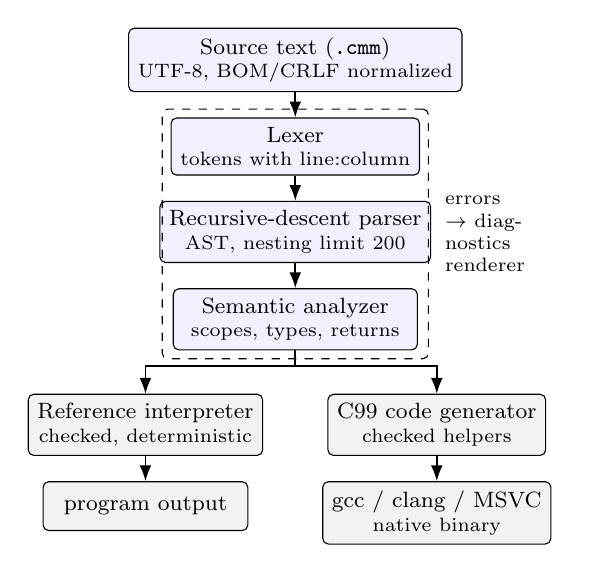
\begin{tikzpicture}[
  font=\footnotesize,
  cmmstage/.style={draw, rounded corners=2pt, fill=blue!6, minimum width=3.1cm, minimum height=0.62cm, align=center},
  cmmout/.style={draw, rounded corners=2pt, fill=gray!10, minimum width=2.6cm, minimum height=0.62cm, align=center},
  arr/.style={-{Latex[length=2mm]}, semithick},
  node distance=0.32cm]
  \node[cmmstage] (src) {Source text (\texttt{.cmm})\\[-1pt]\scriptsize UTF-8, BOM/CRLF normalized};
  \node[cmmstage, below=of src] (lex) {Lexer\\[-1pt]\scriptsize tokens with line:column};
  \node[cmmstage, below=of lex] (par) {Recursive-descent parser\\[-1pt]\scriptsize AST, nesting limit 200};
  \node[cmmstage, below=of par] (ana) {Semantic analyzer\\[-1pt]\scriptsize scopes, types, returns};
  \node[cmmout, below left=0.55cm and -1.15cm of ana] (int) {Reference interpreter\\[-1pt]\scriptsize checked, deterministic};
  \node[cmmout, below right=0.55cm and -1.15cm of ana] (cg) {C99 code generator\\[-1pt]\scriptsize checked helpers};
  \node[cmmout, below=of cg] (cc) {gcc / clang / MSVC\\[-1pt]\scriptsize native binary};
  \node[cmmout, below=of int] (stdout) {program output};
  \draw[arr] (src) -- (lex);
  \draw[arr] (lex) -- (par);
  \draw[arr] (par) -- (ana);
  \draw[arr] (ana.south) -- ++(0,-0.2) -| (int.north);
  \draw[arr] (ana.south) -- ++(0,-0.2) -| (cg.north);
  \draw[arr] (cg) -- (cc);
  \draw[arr] (int) -- (stdout);
  \node[draw, dashed, rounded corners=2pt, fit=(lex)(ana), inner sep=3pt] (fe) {};
  \node[right=0.08cm of fe, align=left, font=\scriptsize, text width=1.35cm] {errors\\$\rightarrow$ diagnostics renderer};
\end{tikzpicture}
\caption{Compiler pipeline. Each stage reports positioned errors to a shared diagnostics renderer.}
\label{fig:pipeline}
\end{figure}

\begin{table}[t]
\caption{Repository structure}
\label{tab:repo}
\centering
\footnotesize
\begin{tabular}{@{}l L{5.4cm}@{}}
\toprule
\textbf{Path} & \textbf{Contents} \\
\midrule
\texttt{cmm/} & Language implementation: 20 modules, 6\,304 lines \\
\texttt{tests/} & 445 tests in 11 files and a corpus of 61 error programs \\
\texttt{web/} & Web studio: HTTP server, page renderer, client application \\
\texttt{docs/} & Normative specification (v0.1 and v0.2), error catalogue, changelog \\
\texttt{examples/} & Example programs with expected output \\
\texttt{extensions/} & VS~Code extension: grammar, language configuration, icons \\
\texttt{case\_studies/} & AVX-512 SIMD predication case study \\
\texttt{scripts/} & Executable builder, documentation and test generators \\
\texttt{paper/} & This report, the IEEE paper and their benchmarks \\
\bottomrule
\end{tabular}
\end{table}

% ======================================================================
\section{Language Specification}\label{sec:lang}
% ======================================================================
\cmm{} is specified normatively in two documents (v0.1.0 and the v0.2.0 addendum) that fix every token,
message, position and output format. A \emph{rule against assumptions} requires the implementation to stop and
ask rather than guess wherever the specification is silent.

\subsection{Design principles}
\emph{(i) Remove rather than guard:} a feature whose misuse causes a vulnerability class is omitted unless it
can be given fully defined semantics. \emph{(ii) No undefined behaviour:} every program has a specified result
or stops with a specified, positioned error. \emph{(iii) Explicitness:} no implicit narrowing, no truthiness,
no context-dependent operators.

\subsection{Lexical structure}
Source files are strict UTF-8; a byte-order mark is removed and CRLF line endings are normalized before
lexing, and columns count Unicode code points. Integer literals are decimal and may not have leading zeros;
float literals need digits on both sides of the point. Strings may use single, double or triple quotes with
six escape sequences. The lexer rejects \texttt{++}, \texttt{--}, single \texttt{\&} and single \texttt{|}
with a hint (L009--L012). There are 25 active keywords and 14 reserved words kept for future versions.

\subsection{Types}
\cmm{} has four primitive types and four generic collections (Table~\ref{tab:types}). Integers are 64-bit and
every operation is range-checked; division truncates toward zero. Floats follow IEEE~754
binary64~\cite{ieee754}, but infinities and NaN can never arise: overflow or division by zero is an error.
The only implicit conversion widens an \texttt{int} operand to \texttt{float} in mixed arithmetic or
comparison; assignment never converts.

\begin{table}[t]
\caption{Types of \cmm{} v0.2.0}
\label{tab:types}
\centering
\footnotesize
\begin{tabular}{@{}l L{5.3cm}@{}}
\toprule
\textbf{Type} & \textbf{Semantics} \\
\midrule
\texttt{int}    & 64-bit signed; overflow traps (R001) \\
\texttt{float}  & IEEE~754 binary64; never Inf or NaN (R002, R004) \\
\texttt{bool}   & \texttt{true}/\texttt{false}; never converted to or from numbers \\
\texttt{string} & immutable Unicode text; indexing by code point, \texttt{.len()} \\
\midrule
\texttt{array<T>} & fixed length, bounds-checked indexing (R006) \\
\texttt{list<T>}  & growable; \texttt{push}, \texttt{pop}, \texttt{insert}, \texttt{remove}, \texttt{contains} \\
\texttt{stack<T>} & LIFO; \texttt{push}, \texttt{pop}, \texttt{peek}; empty pop traps (R012) \\
\texttt{queue<T>} & FIFO; \texttt{enqueue}, \texttt{dequeue}, \texttt{peek} \\
\bottomrule
\end{tabular}
\end{table}

\subsection{Grammar}
Listing~\ref{lst:grammar} gives the core of the v0.2.0 grammar in EBNF. Expressions follow the precedence of
Table~\ref{tab:prec}; all binary operators are left-associative.

\begin{lstlisting}[style=plain,basicstyle=\ttfamily\footnotesize,caption={Core grammar of \cmm{} v0.2.0 (EBNF, abridged).},label={lst:grammar},float=*t]
program    = "module" IDENT ";" function { function } EOF ;
function   = "fn" ( IDENT | "main" ) "(" [ param { "," param } ] ")"
             [ "->" type ] block ;
param      = IDENT ":" type ;
type       = "int" | "float" | "bool" | "string"
           | ( "array" | "list" | "stack" | "queue" ) "<" elemType ">" ;
block      = "{" { statement } "}" ;
statement  = varDecl | assignStmt | callStmt | printStmt | returnStmt
           | ifStmt | whileStmt | doWhileStmt | forStmt | switchStmt | block ;
varDecl    = ( "let" | "mut" ) IDENT "=" expr ";" ;
assignment = IDENT [ "[" expr "]" ] ( "=" | "+=" | "-=" | "*=" | "/=" | "%=" ) expr ;
ifStmt     = "if" "(" expr ")" block [ "else" ( ifStmt | block ) ] ;
forStmt    = "for" "(" forInit [ expr ] ";" [ assignment ] ")" block ;
switchStmt = "switch" "(" expr ")" "{" caseClause { caseClause }
             [ "default" ":" block ] "}" ;
\end{lstlisting}

\begin{table}[t]
\caption{Operator precedence (highest first)}
\label{tab:prec}
\centering
\footnotesize
\begin{tabular}{@{}c l l@{}}
\toprule
\textbf{Level} & \textbf{Operators} & \textbf{Meaning} \\
\midrule
1 & \texttt{a[i]}, \texttt{f(x)}, \texttt{v.m(x)} & postfix: index, call, method \\
2 & \texttt{!}, \texttt{-} & prefix: logical not, negation \\
3 & \texttt{*}, \texttt{/}, \texttt{\%} & multiplicative \\
4 & \texttt{+}, \texttt{-} & additive \\
5 & \texttt{<}, \texttt{<=}, \texttt{>}, \texttt{>=} & comparison \\
6 & \texttt{==}, \texttt{!=} & equality \\
7 & \texttt{\&\&} & logical and (short-circuit) \\
8 & \texttt{||} & logical or (short-circuit) \\
\bottomrule
\end{tabular}
\end{table}

\subsection{Static semantics}
Every variable is declared with \texttt{let} (immutable) or \texttt{mut} (mutable) and must be initialized;
its type is inferred. Conditions must be \texttt{bool}. Assignment is a statement, so \texttt{if (x = 1)} is a
syntax error. Braces are mandatory. Function signatures are collected before bodies are checked, so functions
may be defined in any order. A conservative \emph{definitely-returns} rule rejects a typed function with any
path that does not return (E013). A \texttt{switch} accepts \texttt{int} or \texttt{string} literals, has no
fall-through and rejects duplicate cases.

\subsection{Dynamic semantics}
Assigning, passing or returning a collection copies it deeply, so two names never share data and a callee
cannot modify its caller's variables (Listing~\ref{lst:value}). Immutability is deep: a \texttt{let}
collection allows neither element assignment nor mutating methods. Each call gets a fresh environment
containing only its parameters; there are no globals. Recursion is limited to 1000 nested calls (R007).

\lstinputlisting[language=cmm,caption={Typed functions, a growable list and deep-copy value semantics.},label={lst:value},float=t]{examples/value_semantics.cmm}

% ======================================================================
\section{Compiler Implementation}\label{sec:impl}
% ======================================================================
The implementation is about 6\,300 lines of Python using only the standard library (Table~\ref{tab:loc}).

\begin{table}[t]
\caption{Size of the language implementation}
\label{tab:loc}
\centering
\footnotesize
\begin{tabular}{@{}L{6.4cm} r@{}}
\toprule
\textbf{Component (modules)} & \textbf{Lines} \\
\midrule
Lexer and token definitions (\texttt{lexer}, \texttt{tokens}) & 585 \\
Parser and AST (\texttt{parser}, \texttt{ast\_nodes}) & 1\,343 \\
Semantic analyzer and type rules (\texttt{analyzer}, \texttt{types}) & 778 \\
Interpreter and runtime (\texttt{interpreter}, \texttt{runtime\_*}, \texttt{builtins}) & 1\,117 \\
C99 code generator (\texttt{codegen\_c}) & 859 \\
Diagnostics (\texttt{errors}, \texttt{explanations}, \texttt{suggest}, \texttt{diagnostic\_render}) & 867 \\
CLI and printers (\texttt{cli}, \texttt{astprint}, \texttt{formatting}, others) & 755 \\
\midrule
\textbf{Total} & \textbf{6\,304} \\
\bottomrule
\end{tabular}
\end{table}

\subsection{Lexer}
The hand-written scanner reads the normalized text once, using longest match for operators, and produces
tokens carrying their type, lexeme, value and 1-based line and column. Number literals are validated and
range-checked during scanning (L005--L008). The lexer stops at the first error.

\subsection{Parser}
The parser is a stratified recursive-descent parser~\cite{dragonbook} with one procedure per precedence level
of Table~\ref{tab:prec}, which yields C's usual precedence and left associativity without a separate
precedence table. A statement that begins with an identifier is classified by its next token: call,
method call or assignment. Every nested construct increments a depth counter, and nesting beyond 200 levels
raises S004 instead of overflowing the Python stack.

\subsection{Semantic analyzer}
The analyzer makes two passes. The first records all function signatures and checks them against the
built-in function table; the second walks each body with a stack of lexical scopes, inferring and checking
types, enforcing mutability, validating calls and collection methods against a declarative method table,
checking \texttt{switch} cases and applying the definitely-returns rule. All semantic errors are collected and
reported in source order.

\subsection{Reference interpreter}
The interpreter is a tree-walking evaluator over the verified AST. It defines the language's semantics:
\begin{itemize}
  \item every \texttt{int} result is checked against $[-2^{63}, 2^{63}-1]$ (R001), every float result for
        overflow (R004), and every division and remainder for a zero divisor (R002, R003);
  \item collections are copied on assignment, call and return;
  \item it runs in a thread with a 256\,MB stack, so the 1000-call recursion limit behaves identically on
        every platform;
  \item an optional step budget stops runaway loops (R005); the web server always sets one;
  \item floats are printed with a shortest round-trip algorithm specified in the language definition.
\end{itemize}

\subsection{C99 code generator}
The transpiler lowers the v0.1 subset plus user-defined functions to ISO~C99~\cite{iso_c99} using only
standard headers. Arithmetic becomes calls to small \texttt{static} helpers that perform the interpreter's
overflow and division checks, and a custom float formatter reproduces the interpreter's output exactly.
Collections, indexing and \texttt{switch} are not yet supported; such programs are rejected with T001.

% ======================================================================
\section{Diagnostics}\label{sec:diag}
% ======================================================================
The 60 diagnostic codes (Table~\ref{tab:codes}) are defined in one catalogue, from which the reference
documentation and the golden tests are generated. Every diagnostic has a positioned headline, a source excerpt
with a caret under the offending text, a plain-language explanation and a concrete fix, often with corrected
code. For undeclared names the analyzer suggests the closest declared identifier by Damerau--Levenshtein
distance~\cite{damerau,levenshtein}, allowing one edit for names shorter than five characters and two
otherwise (Listing~\ref{lst:diag}). The \texttt{--no-help} flag restores a terse format for tools.

\begin{table}[t]
\caption{Diagnostic codes by phase}
\label{tab:codes}
\centering
\footnotesize
\begin{tabular}{@{}l l r L{3.85cm}@{}}
\toprule
\textbf{Prefix} & \textbf{Phase} & \textbf{Codes} & \textbf{Examples} \\
\midrule
L & Lexical      & 12 & \texttt{++} not supported, unterminated string \\
S & Syntax       & 3  & expected token, reserved word, nesting \\
E & Semantic     & 30 & undeclared name, \texttt{let} reassigned, missing return \\
R & Runtime      & 14 & overflow, division by zero, index range \\
T & Transpile    & 1  & feature not supported by the C back end \\
\midrule
  & \textbf{Total} & \textbf{60} & \\
\bottomrule
\end{tabular}
\end{table}

\lstinputlisting[style=diag,caption={Diagnostic for a misspelled identifier, as printed by \texttt{cmm run}.},label={lst:diag},float=t]{generated/diag_typo.txt}

% ======================================================================
\section{Developer Tooling}\label{sec:tools}
% ======================================================================
\subsection{Command-line interface}
The \texttt{cmm} command (Table~\ref{tab:cli}) is installed by \texttt{pip} or run as
\texttt{python3 -m cmm}. Output is always UTF-8 with \texttt{\textbackslash n} line endings, and exit codes
distinguish static errors (1), runtime traps (2), I/O errors (3), usage errors (4) and internal errors (70).
A PyInstaller script builds a single-file executable.

\begin{table}[t]
\caption{CLI commands}
\label{tab:cli}
\centering
\footnotesize
\begin{tabular}{@{}l L{4.6cm}@{}}
\toprule
\textbf{Command} & \textbf{Action} \\
\midrule
\texttt{cmm run f [--max-steps N]} & check and execute \\
\texttt{cmm check f} & static checks only \\
\texttt{cmm tokens f} & print the token stream with positions \\
\texttt{cmm ast f} & print the abstract syntax tree \\
\texttt{cmm transpile f -o out.c} & generate ISO C99 \\
\texttt{cmm --version} & print \texttt{cmm 0.2.0} \\
\bottomrule
\end{tabular}
\end{table}

\subsection{Editor support}
A VS~Code extension contributes the \cmm{} language definition, a TextMate grammar for syntax highlighting,
bracket and comment configuration and a file-icon theme. Platform scripts register the \texttt{.cmm} file
type and icon on Windows and macOS.

% ======================================================================
\section{Web Compiler Studio}\label{sec:web}
% ======================================================================
The web studio lets users write and run \cmm{} programs in a browser without installing anything. It is
written with the standard library alone (about 4\,700 lines of Python, JavaScript, HTML and CSS) and is
deployed publicly. Fig.~\ref{fig:web} shows its architecture.

\begin{figure}[t]
\centering
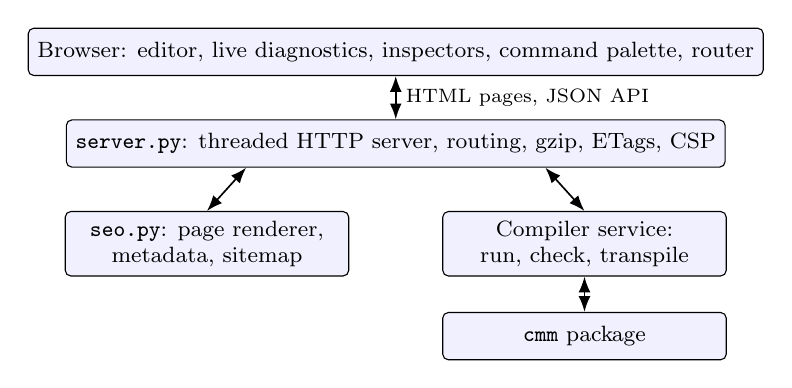
\begin{tikzpicture}[
  font=\footnotesize,
  box/.style={draw, rounded corners=2pt, fill=blue!6, align=center, minimum height=0.6cm},
  arr/.style={{Latex[length=2mm]}-{Latex[length=2mm]}, semithick}]
  \node[box, minimum width=7.6cm] (browser) {Browser: editor, live diagnostics, inspectors, command palette, router};
  \node[box, below=0.55cm of browser, minimum width=7.6cm] (server) {\texttt{server.py}: threaded HTTP server, routing, gzip, ETags, CSP};
  \node[box, below left=0.55cm and -3.6cm of server, minimum width=3.6cm] (seo) {\texttt{seo.py}: page renderer,\\metadata, sitemap};
  \node[box, below right=0.55cm and -3.6cm of server, minimum width=3.6cm] (svc) {Compiler service:\\run, check, transpile};
  \node[box, below=0.45cm of svc, minimum width=3.6cm] (pkg) {\texttt{cmm} package};
  \draw[arr] (browser) -- node[right, font=\scriptsize] {HTML pages, JSON API} (server);
  \draw[arr] (server.south) ++(-1.9,0) -- (seo.north);
  \draw[arr] (server.south) ++(1.9,0) -- (svc.north);
  \draw[arr] (svc) -- (pkg);
\end{tikzpicture}
\caption{Architecture of the web compiler studio.}
\label{fig:web}
\end{figure}

\subsection{Server and API}
The server renders six pages (overview, playground, architecture, pipeline, reference, about) on the server,
so each has its own URL and works without JavaScript. The JSON API (Table~\ref{tab:api}) wraps the compiler
pipeline. Untrusted programs run with a 100\,000-step budget and an empty standard input, request bodies are
limited to 1\,MB, and each request is served on its own thread so that a long-running program cannot block
others.

\begin{table}[t]
\caption{Web studio API}
\label{tab:api}
\centering
\footnotesize
\begin{tabular}{@{}l l L{3.7cm}@{}}
\toprule
\textbf{Method} & \textbf{Endpoint} & \textbf{Result} \\
\midrule
POST & \texttt{/api/run} & output, or diagnostics with failing stage \\
POST & \texttt{/api/check} & static checks only, no execution \\
POST & \texttt{/api/transpile} & generated C99 source \\
POST & \texttt{/api/ast} & formatted syntax tree \\
POST & \texttt{/api/tokens} & token stream with positions \\
GET  & \texttt{/api/presets} & example programs \\
\bottomrule
\end{tabular}
\end{table}

\subsection{Client features}
The editor provides syntax highlighting, automatic indentation, bracket pairing, comment toggling and
diagnostics that update as the user types: errors are marked beside the line numbers and listed in a
Problems panel, and every error location links back to the source. Inspectors show the console output, the
generated C99, the AST and a clickable token table, and a stage trace shows which phase passed or failed.
A command palette, keyboard shortcuts, saved drafts and shareable links complete the interface.

\subsection{Security, performance and discoverability}
Static files are served from an allow-list with path-traversal protection. Every page carries a strict
Content-Security-Policy with a hashed inline script, together with \texttt{nosniff} and referrer-policy
headers. Responses are compressed, and versioned assets are cached immutably. Each page has unique metadata,
Open Graph tags and schema.org structured data, and the server publishes a sitemap and \texttt{robots.txt}.
Lighthouse audits of all six pages scored 97--100 in performance, accessibility, best practices and SEO.

% ======================================================================
\section{Quality Assurance and Deployment}\label{sec:qa}
% ======================================================================
\subsection{Test suite}
Table~\ref{tab:tests} lists the 445 automated tests. The error-help tests run each of the 61 programs in the
error corpus and compare the complete diagnostic with a golden file character for character. The example
tests run every example through the CLI, and the code-generation tests compile the transpiled C99 with
\texttt{-Werror} and require output identical to the interpreter's.

\begin{table}[t]
\caption{Automated tests}
\label{tab:tests}
\centering
\footnotesize
\begin{tabular}{@{}l L{4.3cm} r@{}}
\toprule
\textbf{File} & \textbf{Covers} & \textbf{Tests} \\
\midrule
\texttt{test\_lexer} & tokens, literals, lexical errors & 40 \\
\texttt{test\_parser} & grammar, AST, syntax errors & 46 \\
\texttt{test\_analyzer} & scopes, types, returns & 42 \\
\texttt{test\_interpreter} & semantics, runtime traps & 51 \\
\texttt{test\_v02} & functions, collections, \texttt{switch} & 49 \\
\texttt{test\_formatting} & value and float printing & 26 \\
\texttt{test\_codegen\_c} & C99 back end against interpreter & 16 \\
\texttt{test\_cli} & commands, exit codes, I/O & 39 \\
\texttt{test\_error\_help} & 61 golden diagnostics and helpers & 78 \\
\texttt{test\_examples} & example programs end to end & 30 \\
\texttt{test\_web\_seo} & web server, pages, API & 28 \\
\midrule
\textbf{Total} & & \textbf{445} \\
\bottomrule
\end{tabular}
\end{table}

\subsection{Continuous integration}
GitHub Actions runs the full suite on a matrix of three operating systems (Ubuntu, Windows, macOS) and
three Python versions (3.10, 3.11, 3.12), nine jobs in total, followed by a CLI smoke test. On our
machine 444 of the 445 tests pass. The single failure is a portability defect in the C back end: for a
literal equal to $2^{63}-1$ the generated code prints an \texttt{LL} constant with the \texttt{PRId64}
format, which GCC rejects under \texttt{-Werror} where \texttt{int64\_t} is \texttt{long}. Casting the
constant to \texttt{int64\_t} fixes it.

\subsection{Deployment}
The studio is packaged three ways: a \texttt{Dockerfile} based on \texttt{python:3.12-slim}, a
\texttt{Procfile} for platforms such as Railway, and a \texttt{render.yaml} blueprint. All three install the
package and start \texttt{web/server.py}, which reads its port and public URL from environment variables.
Locally the studio starts with \texttt{python3 web/server.py}.

% ======================================================================
\section{Results and Evaluation}\label{sec:eval}
% ======================================================================
\subsection{Safety guarantees}
Table~\ref{tab:hazards} maps common weakness classes to the \cmm{} rule that removes them and the stage at which a
violating program is stopped. Classes in the upper part cannot be written at all; those in the lower part are
expressible but become deterministic, positioned runtime traps. Every code in the table is exercised by a
program in the test corpus.

\begin{table*}[t]
\caption{Weakness classes and how \cmm{} removes or traps them}
\label{tab:hazards}
\centering
\footnotesize
\begin{tabular}{@{}L{4.4cm} L{8.2cm} L{3.6cm}@{}}
\toprule
\textbf{Weakness (CWE)} & \textbf{\cmm{} rule} & \textbf{Enforced by} \\
\midrule
NULL dereference (CWE-476) & No null value and no pointer types exist & grammar and type system \\
Buffer overflow via pointers (CWE-119, CWE-787) & No address-of, dereference or pointer arithmetic & grammar \\
Use of uninitialized variable (CWE-457) & Every declaration requires an initializer & parser (S001) \\
Use after free, aliasing bugs (CWE-416) & No references; collections are copied on assignment and call & semantics \\
Assignment in condition, \texttt{++}/\texttt{--} misuse & Assignment is a statement; \texttt{++}, \texttt{--}, \texttt{\&}, \texttt{|} rejected & parser, lexer (L009--L012) \\
Implicit conversion, truthiness (CWE-704) & Conditions must be \texttt{bool}; assignment never converts & analyzer (E004, E007) \\
Accidental mutation & \texttt{let} bindings and parameters are deeply immutable & analyzer (E003, E028, E029) \\
Switch fall-through (CWE-484) & No fall-through; duplicate cases rejected & semantics, analyzer (E023) \\
\midrule
Out-of-bounds index (CWE-125, CWE-787) & Every index is checked & runtime trap (R006) \\
Integer overflow (CWE-190) & All \texttt{int} operations checked in 64 bits & runtime trap (R001) \\
Division by zero (CWE-369) & Checked for \texttt{/} and \texttt{\%} on both types & runtime trap (R002, R003) \\
Uncontrolled recursion (CWE-674) & Depth limited to 1000 calls on every platform & runtime trap (R007) \\
\bottomrule
\end{tabular}
\end{table*}

\subsection{Performance}
Table~\ref{tab:perf} reports two experiments on four benchmarks: recursion, integer loops with division,
data-dependent control flow and floating point. The first compares the interpreter with the same program
transpiled to C99 and compiled with \texttt{gcc -O2}; \benchAllMatch{} between the two back ends. The second
measures the cost of the safety checks by comparing the transpiled C99 with hand-written, unchecked C. Times
are the best of several runs on \benchCPU{}, with GCC \benchCC{} and Python \benchPython{}. Native times
include process start-up, which dominates in Experiment~1, so its speedups are lower bounds.

\begin{table*}[t]
\caption{Performance: interpreter vs.\ transpiled C99, and checked C99 vs.\ unchecked hand-written C}
\label{tab:perf}
\centering
\footnotesize
\begin{tabular}{@{}l r r r r r r r r@{}}
\toprule
 & \multicolumn{4}{c}{\textbf{Experiment 1: execution back ends}} & \multicolumn{4}{c}{\textbf{Experiment 2: cost of checks}} \\
\cmidrule(lr){2-5}\cmidrule(l){6-9}
\textbf{Benchmark} & $N$ & \textbf{Interp. (s)} & \textbf{C99 (ms)} & \textbf{Speedup} & $N$ & \textbf{Checked C99 (s)} & \textbf{Plain C (s)} & \textbf{Overhead} \\
\midrule
\inputrows{generated/bench_rows.tex}
\bottomrule
\end{tabular}
\end{table*}

The transpiled C99 is \benchSpeedupMin--\benchSpeedupMax\,$\times$ faster than the interpreter, whose purpose
is to define the semantics rather than to be fast. The checked C99 is \benchOverheadMin--\benchOverheadMax\%
slower than unchecked C; this is the price of the guarantees. The cost is lowest when work is dominated by
control flow (Collatz) and highest for recursive Fibonacci and the floating-point series, whose every division
and result is checked.

\subsection{Case study: modelling SIMD predication}
To test \cmm{} as a modelling tool, we used it to study a classic vectorization problem: a loop computing
\texttt{B[i] = A[i] > 0 ? sqrt(A[i]) : 0}. A \cmm{} program modelled 512-bit AVX-512 registers as 16-lane
\texttt{array<float>} values and mask registers as \texttt{array<bool>} values. It executed the loop four ways
(scalar with a branch, AVX-512 masked, AVX-512 using \texttt{max}, AVX2 blend) and verified lane by lane that
all four agree. It also simulated a 2-bit and a two-level branch predictor and estimated instruction counts.

A hardware benchmark on an Intel Xeon with AVX-512 confirmed the model: predication removed every
data-dependent branch, cut dynamic instructions per element by about $18\text{--}21\times$ (8 to
0.375--0.44) and branches by $32\times$, and made the loop about $19\times$ faster on random data while its run
time became independent of the data. One finding was specific to \cmm{}: removing the tail mask
from a modelled load made the program stop with R006 instead of reading past the array, the very fault that
hardware masked loads exist to prevent~\cite{ifconversion}.

% ======================================================================
\section{Limitations and Future Work}\label{sec:future}
% ======================================================================
\begin{itemize}
  \item \textbf{Expressiveness:} no structs, enumerations, maps, nested collections, first-class functions or
        string concatenation. User-defined record types are the next planned feature.
  \item \textbf{Copy cost:} deep-copying collections is expensive for large data; copy-on-write would keep
        the semantics at lower cost.
  \item \textbf{C99 back end:} collections, indexing and \texttt{switch} are not yet supported, and the
        \texttt{PRId64} portability defect should be fixed.
  \item \textbf{Check overhead:} static range analysis could remove checks that can never fail.
  \item \textbf{Interpreter speed:} a bytecode virtual machine would be considerably faster than tree walking.
  \item \textbf{Verification:} a formal semantics would allow the interpreter to be verified against it.
\end{itemize}

% ======================================================================
\section{Conclusion}
% ======================================================================
This project designed and implemented \cmm{}, a small imperative language that obtains memory safety and
freedom from undefined behaviour by removing dangerous features rather than adding protective machinery.
The deliverables are a normative specification, a dependency-free toolchain with two execution back ends,
beginner-friendly diagnostics, a CLI, an editor extension and a deployed web studio, validated by 445 tests on
three operating systems. The evaluation shows that the most common weakness classes either cannot be written
in \cmm{} or stop deterministically with a clear explanation, at a measurable but moderate run-time cost in the
compiled output. The source code, documentation and studio are openly available~\cite{cmm_repo}.

\section*{Acknowledgment}
The authors thank Prof.\ Hariharan R L, Center for AI Research, School of Computer Science and Engineering
(SCOPE), for his guidance and supervision throughout this project.

\bibliographystyle{IEEEtran}
\bibliography{references}

\end{document}
